%!TEX root = thesis.tex


\chapter{SWEET-Cat}
\label{sec:SWEET-Cat}

Part of the work during the thesis has been dedicated to regularly update
SWEET-Cat\footnote{\url{https://www.astro.up.pt/resources/sweet-cat/}}, a catalogue with all
discovered planet hosts, and the stellar parameters.

In this chapter a detailed description of SWEET-Cat will be presented. Moreover an analysis of 50
planet hosts was performed during the thesis with updated planetary parameters (mass and radius).


\section{What is SWEET-Cat?}

As mentioned above, SWEET-Cat is a catalogue of planet host stars. However, the strength of
SWEET-Cat is the homogeneously analysed stars utilising the method described in
\sref{sec:parameters} with \code{FASMA} or a similar tool before the creation of \code{FASMA}.

In the era with a large number of discovered exoplanets (more than 3500 confirmed exoplanet at the
moment of writing), the time for in-depth statistical studies has arrived. However, when conducting
these studies it is crucial to have consistent measurements of e.g. stellar atmospheric parameters.
This can be obtained by using a single analysis to obtain these parameters, as it is know that
different methods will lead to different results \citep[see e.g.][for a recent review]{Hinkel2016}.

To obtain stellar atmospheric parameters from one method is an on-going goal with SWEET-Cat, where
high quality spectra are obtained for stars hosting planets. These are used to determine the stellar
parameters in a homogeneous way. All stars in SWEET-Cat analysed with the method from our group are
marked with a flag showing whether it is analysed homogeneously or not. The columns provided in
SWEET-Cat are summarised in \tref{tab:sweetcat}. It is important to note that SWEET-Cat does not
include any planetary parameters.

\begin{table}[htb!]
    \caption{Columns in SWEET-Cat}
    \label{tab:sweetcat}
    \centering
    \begin{tabular}{lrl}
      \hline\hline
      Column                         & Unit      & Description \\
      \hline
      Name                           &           & Popular stellar name                                 \\
      HD number                      &           & HD number                                            \\
      RA                             & \si{deg}  & Right ascension                                      \\
      Dec                            & \si{deg}  & Declination                                          \\
      $\mathrm{Vmag}$                & \si{mag}  & V magnitude                                          \\
      $\sigma(\mathrm{Vmag})$        & \si{mag}  & Error on V magnitude                                 \\
      $\pi$                          & \si{mas}  & Parallax                                             \\
      $\sigma(\pi)$                  & \si{mas}  & Error on parallax                                    \\
      Source of $\pi$                &           & Source of parallax measurement                       \\
      $T_\mathrm{eff}$               & \si{K}    & Effective temperature                                \\
      $\sigma(T_\mathrm{eff})$       & \si{K}    & Error on effective temperature                       \\
      $\log g$                       & \si{dex}  & Surface gravity                                      \\
      $\sigma(\log g)$               & \si{dex}  & Error on surface gravity                             \\
      $\log g_{\mathrm{LC}}$         & \si{dex}  & Surface gravity corrected from light curves          \\
      $\sigma(\log g_{\mathrm{LC}})$ & \si{dex}  & Error on surface gravity corrected from light curves \\
      $\xi_\mathrm{micro}$           & \si{km/s} & Micro turbulence                                     \\
      $\sigma(\xi_\mathrm{micro})$   & \si{km/s} & Error on micro turbulence                            \\
      $[\ion{Fe}/\ion{H}]$           & \si{dex}  & Metallicity                                          \\
      $\sigma([\ion{Fe}/\ion{H}])$   & \si{dex}  & Error on metallicity                                 \\
      Mass                           & $M_\odot$ & Stellar mass                                         \\
      $\sigma(\mathrm{Mass})$        & $M_\odot$ & Error on stellar mass                                \\
      Reference                      &           & Reference for parameters                             \\
      Homogeneity flag               & 0/1       & 0 for not homogeneous analysis, 1 otherwise          \\
      Last updated                   & date      & Last updated                                         \\
      Comments                       &           & Any special remarks/comments (e.g. M star)           \\
      \hline
    \end{tabular}
\end{table}

SWEET-Cat is updated on a weekly basis if new planet hosts are discovered, and whenever planet hosts
have been analysed with the method from our group, as described in this thesis.


\section{Data for 50 planet hosts}

In this section the data for a large update to SWEET-Cat will be described. The majority of the data
comes as a result from proposals submitted for observational time, while some of the data was found
in the archive. In the next section the analysis of the 50 spectra will be presented along with the
results.


\subsection{Proposals for observation time}



\subsection{Data collected from proposals}



\subsection{Data collected from archive}



\section{Analysis}


The method of determining atmospheric parameters from the curve of growth analysis has been applied
several times in the optical \citep[see e.g.][]{Mortier2013b,Tsantaki2013,Sousa2011,Santos2013}.
When studying stars with planets and any correlations between stellar and planetary parameters it is
important to have a homogeneous characterisation of the stars. An effort to create such a sample was
initiated by \citet{Santos2013} with the SWEET-Cat database. The motivation to homogenise the
stellar hosts is mainly to compare the hosts and make statistical studies on one consistent scale.
When doing these statistical studies, the results might otherwise suffer from offsets between
different methods.

The skills acquired during the NIR studies as mentioned above were directly translated into deriving
parameters for a sample of 50 known planet host stars that were not previously analysed by our group
\citep{Andreasen2017a}. The spectra of these stars were required at UVES, FIES, HARPS, and ESPaDOnS
with the mean S/N higher than 200\unfinished{Write more about the data acquisition here}.

A Hertzsprung-Russell diagram of the sample can be seen in \fref{fig:sweetcat}. The sample covers a
large range of $T_\mathrm{eff}$, FGK, while there are both dwarf, sub-giant, and some giant stars.
The colours indicate the $\log g$. In order to determine the luminosity of each star the simple
relation
\begin{align*}
  L = 4\pi R^2 \sigma T^4_\mathrm{eff}
\end{align*}
is used, where $L$ is the luminosity, $R$ is the stellar radius, and $\sigma$ is the
Stefan-Boltzmann constant. In solar units this relation is simply:
\begin{align*}
  \frac{L}{L_\odot} = \left(\frac{R}{R_\odot}\right)^2 \left(\frac{T_\mathrm{eff}}{T_{\mathrm{eff},\odot}}\right)^4
\end{align*}
In order to determine the the stellar radius, the empirical relation from \citet{Torres2010} was
used.

\begin{figure}[htpb!]
    \centering
    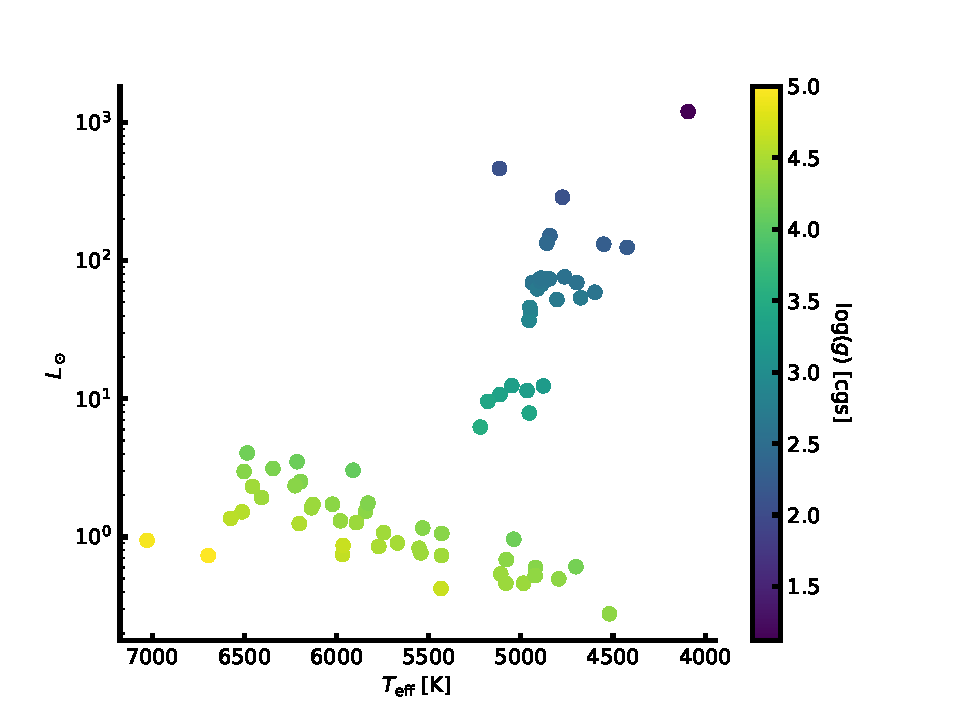
\includegraphics[width=1.0\linewidth]{figures/HR.pdf}
    \caption{A Hertzsprung-Russell diagram of the sample of 50 planet host stars added to SWEET-Cat.
             The parameters were derived using optical high resolution and high S/N spectra in
             tandem with \code{FASMA} and an optical line list. The colour scale shows the derived
             $\log g$ for each star.}
    \label{fig:sweetcat}
\end{figure}

The parameters were derived using \code{FASMA} with the optical line list compiled by
\citet{Sousa2008a} and \citet{Tsantaki2013} for stars where $T_\mathrm{eff}$ was below \SI{5200}{K}.
All the new derived parameters were added to SWEET-Cat, available for the community.

With these updated parameters the completeness of SWEET-Cat for stars brighter than V magnitude 10
is 85\% (77\% for stars brighter than 12). For fainter stars it is time expensive to acquire spectra
of the quality needed for this method. Moreover, many of the fainter planet host stars have been
observed with the \emph{Kepler} space mission, where most stars are faint.

SWEET-Cat was recently combined with planetary masses to see two distinctive populations for giant
planets by \citet{Santos2017}. This can be seen in the mass histogram in \fref{fig:giantpopulations}
for the full sample of giant planets, with masses higher than 1 Jupiter mass and lower than 20
Jupiter masses, and for a sample constrained by: $\SI{4000}{K}\leq T_\mathrm{eff} \leq\SI{6500}{K}$
in order to have reliably atmospheric parameters from spectroscopic data, orbital periods above
\SI{10}{days} to avoid hot jupiters whose formation and migration process is debated \citep[see
e.g.]{Ngo2016}, orbital periods below 5 years to allow for the sample to be reasonable complete.
Last only stars brighter than 13 magnitude were included to ensure that the planetary masses can
have been derived with reasonable confidence using the radial velocities.

\begin{figure}[htpb!]
    \centering
    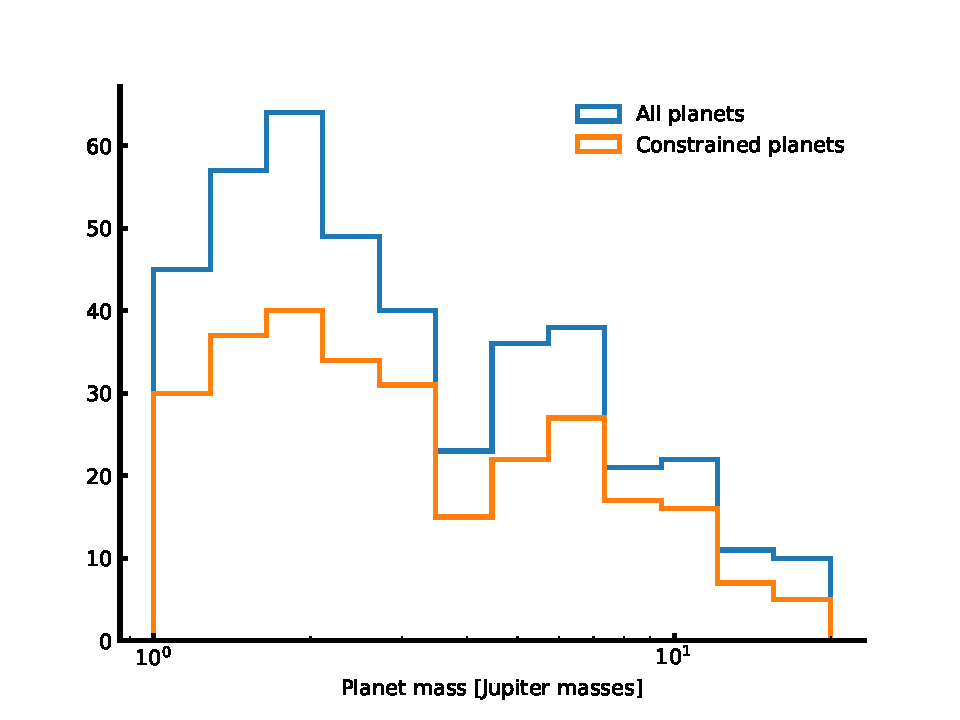
\includegraphics[width=1.0\linewidth]{figures/giantPopulation.pdf}
    \caption{Giant planet masses for the full sample and constrained sample (see text for details).
             This study was performed by \citet{Santos2017} to distinct two giant planet populations.}
    \label{fig:giantpopulations}
\end{figure}

By separating the distribution into two at $4M_{Jup}$, it can be shown \citep[see][for
details]{Santos2017} that the stars hosting the more massive giant planets are in average more
metal-poor compared to the stars hosting the lower mass giant planets. This suggest two different
stellar populations forming giant planets.


\section{Future work}
